\documentclass[12pt]{article}

\usepackage[a4paper,margin=1in]{geometry}
\usepackage[utf8]{inputenc}
\usepackage[spanish,es-tabla]{babel}
\usepackage{graphicx}
\usepackage{circuitikz}
\usepackage{amsmath}
\usepackage{subcaption}
\usepackage{amssymb}
\usepackage[hidelinks]{hyperref}
\usepackage{mathtools}
%\usepackage[table,xcdraw]{xcolor}
\usepackage{enumitem}
\usepackage{array}
\usepackage{longtable}
\usepackage{multirow}
\usepackage{csquotes}
\usepackage{float}
\usepackage{setspace}
\usepackage{pgfplots}
\pgfplotsset{compat=1.18}
\usetikzlibrary{arrows.meta, decorations.pathreplacing, calc, positioning}
\usepackage[style=ieee, backend=bibtex]{biblatex}
\addbibresource{bibliografía.bib}
\graphicspath{{Figuras/}}
\onehalfspacing

\hypersetup{
    colorlinks=true,
    linkcolor=blue,    
    citecolor=blue,
    urlcolor=blue,
    filecolor=blue
}

\begin{document}       
\renewcommand{\figureautorefname}{Fig.}
\renewcommand{\tableautorefname}{Tab.}
\renewcommand{\equationautorefname}{Ec.}

\begin{titlepage}
\thispagestyle{empty}
\begin{tikzpicture}[remember picture,overlay]
    \node[opacity=0.2,anchor=center] at (current page.center) 
        {
\includegraphics[width=0.9\paperwidth]{decoracion_a.png}};
\end{tikzpicture}
\begin{center}
    
\includegraphics[width=15cm]{unc_fcefyn_logo.png} \\ [0.5cm]
    \LARGE Universidad Nacional de Córdoba \\ [0.5cm] 
    \large Facultad de Ciencias Exactas, Físicas y Naturales \\ 
    \vspace{40pt}
    \large Sistemas de Radiocomunicación \\ [0.2cm]
    \large Trabajo Práctico N°4 \\
    \vspace{60pt}
    \LARGE Enlaces Punto a Punto con Fibra Óptica\\
    \vspace{60pt}
    \begin{table}[!h]
        \centering
        \begin{tabular}{ll}
            \multicolumn{1}{c}{Nombre} & \multicolumn{1}{c}{DNI} \\
            Mendes Rosa, Agustín             & 44.517.201 \\
            Monja, Ernesto Joaquín           & 43.873.728 \\
            Arteaga Barrera, Cristian Eduardo           & 95.159.096 \\
            Baccino, Luca           & 45.328.380 
        \end{tabular}
    \end{table}
    \vspace{20pt}
    \begin{table}[!h]
        \centering
        \begin{tabular}{ll}
            \multicolumn{1}{c}{Docentes} & Esp. Ing. Liendo, Carlos Guillermo \\
                                         & Ing. Dadam, Federico Tomás \\
        \end{tabular}
    \end{table}
    \vfill
        {\small Córdoba, República Argentina\\
                Año 2026}
\end{center}
\end{titlepage}
\newpage

\tableofcontents
\newpage
\listoffigures
\newpage
\listoftables
\newpage

\section{Introducción}
\label{sec_1}
El presente trabajo práctico aborda el diseño, dimensionamiento y validación técnica de un enlace de fibra óptica punto a punto de $8 \, [km]$ de longitud, proyectado para operar a una tasa de transmisión de $1 \, [Gbps]$ en la ventana óptica de $1310 \, [nm]$. El sistema emplea una topología bidireccional mediante el uso de $2$ fibras ópticas monomodo instaladas en canalización subterránea, garantizando el aislamiento y la integridad de la señal frente a condiciones ambientales adversas.

El objetivo central radica en determinar la viabilidad del enlace mediante la selección fundamentada del equipamiento activo y pasivo, la construcción del presupuesto de potencia óptica y el análisis de los márgenes de seguridad requeridos. A través de la caracterización de cada evento físico (atenuación intrínseca de la fibra, pérdidas por inserción en conectores y empalmes por fusión), se establece la factibilidad técnica y operativa del enlace proyectado.

El trabajo se organiza siguiendo las partes de la consigna. En la \autoref{sec_2} se seleccionan el transceptor, la fibra, los conectores y empalmes y los distribuidores ópticos, considerando tanto criterios técnicos como económicos. En la \autoref{sec_3} se calcula el presupuesto de potencia y se verifica la viabilidad del enlace. En la \autoref{sec_4} se representa gráficamente el enlace con cada evento de pérdida y la evolución del nivel de potencia. Finalmente, en la \autoref{sec_5} se responden las preguntas de análisis sobre la extensión del enlace, el uso de la ventana de $1550 \, [nm]$, el margen de seguridad y los instrumentos de validación.


\section{Selección de Elementos}
\label{sec_2}
Para el dimensionamiento del enlace óptico punto a punto de $8 \, [km]$, se seleccionan los componentes activos y pasivos respetando las normativas de la \textit{UIT-T} y los estándares de la industria de telecomunicaciones.


\subsection{Transceptor Óptico (SFP)}
Se selecciona un módulo transceptor del tipo \textbf{SFP 1000BASE-LX}, modelo \textit{ProLabs SFP-1000BASE-LX-I-C}, el cual trabaja a $1310 \, [nm]$ sobre fibra monomodo con conector \textit{LC} dúplex, es decir, utiliza una fibra para transmisión y otra para recepción, tal como requiere el enlace. Según su hoja de datos \cite{b1}, presenta los parámetros técnicos de la \autoref{fig:fig_1} y la \autoref{fig:fig_2}:
\begin{figure}[H]
    \centering
    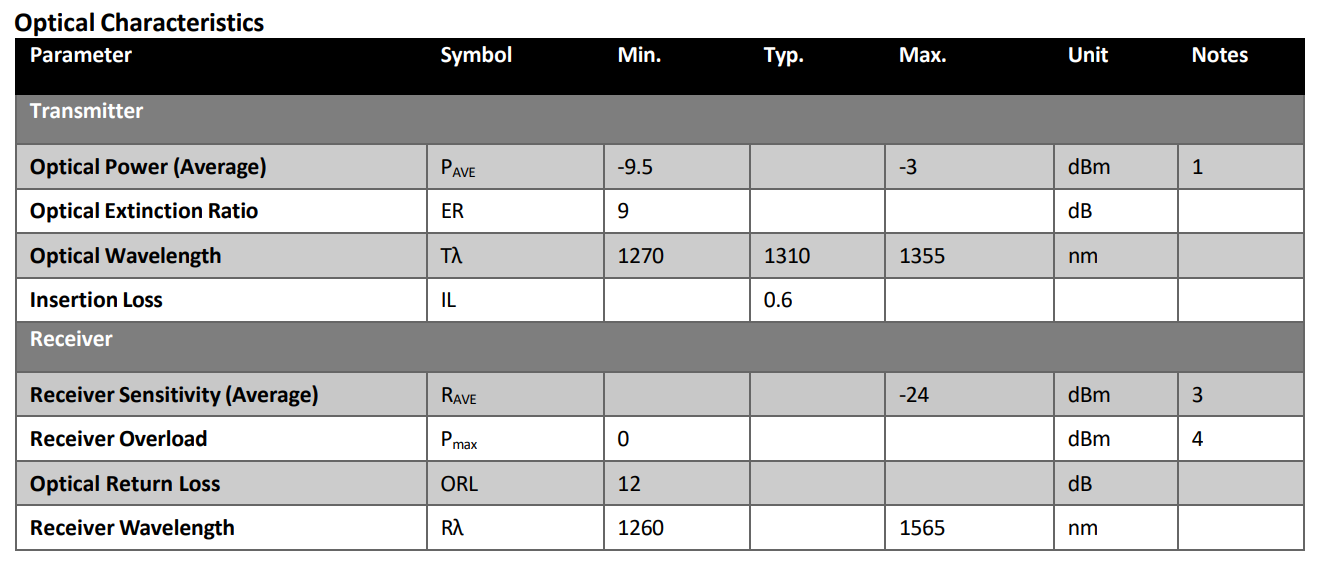
\includegraphics[width=0.8\textwidth]{Figura 1.png}
    \caption{Características ópticas del transceptor SFP 1000BASE-LX. Fuente: Hoja de datos del fabricante \cite{b1}.}
    \label{fig:fig_1}
\end{figure}

\begin{figure}[H]
    \centering
    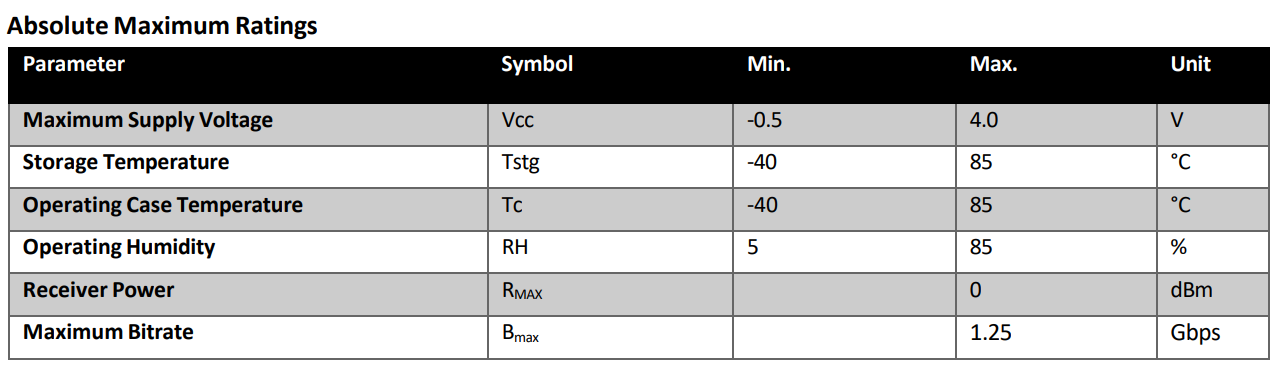
\includegraphics[width=0.8\textwidth]{Figura 2.png}
    \caption{Valores máximos absolutos del transceptor SFP 1000BASE-LX. Fuente: Hoja de datos del fabricante \cite{b1}.}
    \label{fig:fig_2}
\end{figure}

De las figuras se extraen los siguientes parámetros de operación:
\begin{itemize}
    \item \underline{Longitud de onda de operación ($\lambda$):} $1310 \, [nm]$ (rango de $1270$ a $1355 \, [nm]$).
    \item \underline{Potencia de transmisión ($P_{t}$):} mínima de $-9.5 \, [dBm]$ y máxima de $-3 \, [dBm]$.
    \item \underline{Sensibilidad del receptor ($S_r$):} $-24 \, [dBm]$.
    \item \underline{Potencia de sobrecarga del receptor ($P_{sat}$):} $0 \, [dBm]$.
    \item \underline{Tasa máxima:} $1.25 \, [Gbps]$, suficiente para \textit{Gigabit Ethernet} ($1 \, [Gbps]$ de datos con codificación 8B/10B).
\end{itemize}

El \textit{Optical Budget} (presupuesto óptico) es la máxima atenuación que puede introducir el trayecto para que la señal llegue al receptor con un nivel igual a su sensibilidad. Siguiendo un criterio conservador, se calcula con la potencia de transmisión mínima garantizada por el fabricante \cite{b7}:
\begin{equation}
    OB = P_{t,min} - S_r = -9.5 \, [dBm] - (-24 \, [dBm]) = 14.5 \, [dB]
    \label{eq:optical_budget}
\end{equation}

Si se utilizara la potencia máxima, el presupuesto sería de $21 \, [dB]$; sin embargo, ese valor describe el caso favorable y no garantiza el funcionamiento del enlace, por lo que se adopta $OB = 14.5 \, [dB]$ para el diseño.

\textbf{Justificación:} el estándar 1000BASE-LX cubre la distancia de $8 \, [km]$ a $1310 \, [nm]$, longitud de onda que coincide con la zona de dispersión cromática prácticamente nula de las fibras monomodo estándar, por lo que el enlace queda limitado únicamente por atenuación.


\subsection{Fibra Óptica}
\subsubsection{Tipo de fibra: G.652.D frente a G.657}
La consigna plantea elegir entre dos tipos de fibra monomodo:
\begin{itemize}
    \item \underline{UIT-T G.652.D} \cite{b5}: fibra monomodo estándar de bajo pico de agua (\textit{Low Water Peak}), optimizada para $1310 \, [nm]$ y utilizable en todo el rango de $1260$ a $1625 \, [nm]$. Es la fibra de uso general en redes troncales y de transporte.
    \item \underline{UIT-T G.657} \cite{b6}: fibra monomodo insensible a curvaturas (\textit{bend-insensitive}). La categoría G.657.A es compatible con G.652.D, pero admite radios de curvatura mucho menores (de $10$ a $7.5 \, [mm]$), por lo que se emplea principalmente en instalaciones internas, acometidas FTTH y cajas con poco espacio.
\end{itemize}

Ambas presentan una atenuación similar a $1310 \, [nm]$, por lo que la diferencia está en la aplicación. Se selecciona la \textbf{fibra G.652.D}, ya que el enlace es un tramo troncal de $8 \, [km]$ en ducto subterráneo, donde el cable se instala respetando radios de curvatura amplios y la ventaja de la G.657 frente a macrocurvaturas no aporta beneficios que justifiquen su mayor costo. Además, es la fibra recomendada por la bibliografía de la cátedra para este tipo de enlaces \cite{b7}.

\subsubsection{Cable seleccionado}
Se adopta el cable \textbf{Lightera CFOA-SM-DDR-S 04F TS G-652D (PFV) NR}, cable óptico dieléctrico totalmente seco para ductos, con protección dieléctrica contra roedores, fabricado según la norma ABNT NBR 14773 \cite{b2}:
\begin{itemize}
    \item \underline{Fibras:} 4 fibras monomodo G.652.D, de las cuales 2 se utilizan para el enlace (transmisión y recepción) y 2 quedan de reserva para mantenimiento o futuras ampliaciones.
    \item \underline{Atenuación ($\alpha$):} $0.38 \, [dB/km]$ máxima a $1310 \, [nm]$. La especificación del cable remite las características ópticas a la especificación de fibra monomodo del fabricante; el valor adoptado es la atenuación máxima que Lightera declara para fibra G.652.D cableada \cite{b3}. Se utiliza el valor máximo para el cálculo conservador del presupuesto.
    \item \underline{Estructura:} tubos holgados (\textit{loose tube}) con núcleo totalmente seco protegido contra la humedad mediante materiales hidroexpansibles, elemento central de FRP (plástico reforzado con fibra de vidrio), filamentos dieléctricos de tracción, capa interna termoplástica, capa de fibra de vidrio de $1.3 \, [mm]$ contra roedores y cubierta externa de polietileno negro resistente a la intemperie. Diámetro nominal de $12.4 \, [mm]$ y masa de $127 \, [kg/km]$.
    \item \underline{Características mecánicas:} carga máxima de instalación de $2000 \, [N]$ y compresión de $1000 \, [N]$; radio mínimo de curvatura de $20$ veces el diámetro durante la instalación y $10$ veces una vez instalado; temperatura de operación de $-20$ a $65 \, [^\circ C]$.
    \item \underline{Presentación:} bobinas de $4000 \, [m]$, por lo que el tramo de $8 \, [km]$ requiere necesariamente empalmes intermedios, lo cual es coherente con las cajas de empalme previstas en la ruta.
\end{itemize}

\textbf{Justificación:} al ser totalmente dieléctrico, el cable es inmune a inducciones y descargas eléctricas y no requiere puesta a tierra. Su núcleo seco protegido contra la penetración de agua y su resistencia a la tracción lo hacen apto para ser tendido en ductos subterráneos, donde puede quedar expuesto a humedad o inundaciones y es sometido a esfuerzos durante el tirado. La capa de fibra de vidrio lo protege contra el ataque de roedores, un riesgo habitual en canalizaciones subterráneas, sin agregar elementos metálicos.


\subsection{Conectores y Empalmes}
Todos los conectores son del tipo \textit{LC/UPC}, compatibles con el transceptor seleccionado. Considerando el recorrido de una fibra (un sentido de transmisión), desde el SFP del \textit{Router A} hasta el SFP del \textit{Router B}, se tienen los siguientes elementos:
\begin{itemize}
    \item \underline{Patchcords ($2$):} uno en cada extremo, entre el SFP y el panel del ODF. Cada patchcord tiene $2$ conectores LC/UPC, uno hacia el SFP y otro hacia el adaptador del ODF.
    \item \underline{Adaptadores de panel ($2$):} uno en cada ODF, donde se acopla el patchcord con el pigtail.
    \item \underline{Pigtails ($2$):} uno en cada ODF. Tienen un conector LC/UPC que se inserta en el adaptador y su otro extremo se empalma por fusión con la fibra del cable exterior.
    \item \underline{Empalmes por fusión ($4$):}
    \begin{enumerate}
        \item 1 empalme en el \textit{ODF A} (pigtail con fibra del cable exterior).
        \item 2 empalmes en las cajas de empalme subterráneas intermedias, que dividen el tendido en 3 tramos de cable.
        \item 1 empalme en el \textit{ODF B} (fibra del cable exterior con pigtail).
    \end{enumerate}
\end{itemize}

En total, cada fibra atraviesa $6$ conectores LC/UPC ($4$ de los patchcords y $2$ de los pigtails), $2$ adaptadores y $4$ empalmes por fusión. Como el enlace es bidireccional con dos fibras, la cantidad de elementos físicos a instalar es el doble, pero el presupuesto se calcula por sentido, ya que ambas fibras recorren el mismo trayecto.

Las pérdidas asignadas a cada elemento, tomadas de los valores típicos de la bibliografía \cite{b7}, se resumen en la \autoref{tab:perdidas_elementos}.

\begin{table}[H]
    \centering
    \caption{Pérdidas típicas asignadas a cada elemento del enlace.}
    \label{tab:perdidas_elementos}
    \begin{tabular}{|l|c|c|}
        \hline
        \textbf{Elemento} & \textbf{Cantidad por fibra} & \textbf{Pérdida unitaria} \\
        \hline
        Fibra G.652.D a $1310 \, [nm]$ & $8 \, [km]$ & $0.38 \, [dB/km]$ \\
        Patchcord LC/UPC (2 conectores) & $2$ & $0.4 \, [dB]$ \\
        Pigtail LC/UPC & $2$ & $0.2 \, [dB]$ \\
        Adaptador de panel LC/UPC & $2$ & $0.15 \, [dB]$ \\
        Empalme por fusión & $4$ & $0.1 \, [dB]$ \\
        \hline
    \end{tabular}
\end{table}


\subsection{Distribuidor Óptico (ODF)}
En cada extremo del enlace (\textit{Sitio A} y \textit{Sitio B}) se instala un distribuidor interno óptico \textbf{Lightera DIO BW12} \cite{b4}, en el cual termina el cable exterior. Sus características principales son:
\begin{itemize}
    \item \underline{Capacidad:} hasta $12$ empalmes en una bandeja articulada reversible, suficiente para las $4$ fibras del cable (las $2$ activas y las $2$ de reserva).
    \item \underline{Acceso:} placa de hasta $12$ adaptadores LC dúplex, compatible con los conectores LC/UPC del enlace.
    \item \underline{Cable de entrada:} admite cables \textit{loose tube} de hasta $14 \, [mm]$ de diámetro, por lo que acepta el cable CFOA-SM-DDR de $12.4 \, [mm]$, y cuenta con un elemento de fijación para los elementos de tracción del cable.
    \item \underline{Instalación:} montaje en rack de $19"$ o sobre superficie, en ambiente interno.
\end{itemize}

\textbf{Justificación:} el ODF actúa como punto de demarcación y transición entre el cable exterior de estructura holgada y los patchcords flexibles que conectan a los SFP. Protege mecánicamente los empalmes por fusión, organiza las fibras de reserva y simplifica las tareas de prueba, mantenimiento y reconfiguración del enlace.

\newpage



\section{Cálculo del Presupuesto de Potencia}
\label{sec_3}
El cálculo del presupuesto de potencia permite verificar matemáticamente si la señal óptica emitida por el transceptor emisor llegará al receptor con un nivel de potencia adecuado, superando su sensibilidad y garantizando un margen de seguridad frente a futuras degradaciones del enlace.


\subsection{Parámetros de Diseño y Ecuaciones Base}
\label{sec_3_1}
A partir de la selección de componentes realizada en la \autoref{sec_2}, se definen los parámetros de entrada para el cálculo del enlace:
\begin{itemize}
    \item \underline{Longitud del enlace ($L$)}: $8.0 \, [km]$
    \item \underline{Longitud de onda ($\lambda$)}: $1310 \, [nm]$
    \item \underline{Potencia de transmisión mínima ($P_{t}$)}: $-9.50 \, [dBm]$
    \item \underline{Sensibilidad del receptor ($S_{r}$)}: $-20.00 \, [dBm]$
    \item \underline{Atenuación específica de la fibra ($\alpha$)}: $0.35 \, [dB/km]$ (G.652.D a $1310 \, [nm]$)
    \item \underline{Pérdida por conector ($A_{c}$)}: $0.30 \, [dB]$ por acople \textit{LC/UPC} ($N_{c} = 4$)
    \item \underline{Pérdida por empalme ($A_{e}$)}: $0.10 \, [dB]$ por fusión ($N_{e} = 4$)
\end{itemize}

Las ecuaciones fundamentales del presupuesto óptico de potencia son:
\begin{equation}
    A_{total} = (L \cdot \alpha) + (N_{c} \cdot A_{c}) + (N_{e} \cdot A_{e})
    \label{eq_1}
\end{equation}

\begin{equation}
    P_{r} = P_{t} - A_{total}
    \label{eq_2}
\end{equation}

\begin{equation}
    M_{s} = P_{r} - S_{r}
    \label{eq_3}
\end{equation}


\subsection{Cálculo Detallado de Atenuación del Canal}
\label{sec_3.2}
\begin{enumerate}
    \item \underline{Pérdida en la fibra óptica ($A_{\text{fibra}}$)}:
    \begin{equation}
        A_{fibra} = 8.0 \, [km] \times 0.35 \, \left[\frac{dB}{km}\right] = 2.80 \, [dB]
        \label{eq_4}
    \end{equation}
    
    \item \underline{Pérdida total por conectores ($A_{conectores}$)}:
    \begin{equation}
        A_{conectores} = 4 \times 0.30 \, [dB] = 1.20 \, [dB]
        \label{eq_5}
    \end{equation}
    
    \item \underline{Pérdida total por empalmes de fusión ($A_{empalmes}$)}:
    \begin{equation}
        A_{empalmes} = 4 \times 0.10 \, [dB] = 0.40 \, [dB]
        \label{eq_6}
    \end{equation}
    
    \item \underline{Atenuación total acumulada ($A_{total}$)}:
    \begin{equation}
        A_{total} = 2.80 \, [dB] + 1.20 \, [dB] + 0.40 \, [dB] = 4.40 \, [dB]
        \label{eq_7}
    \end{equation}
\end{enumerate}


\subsection{Nivel de Potencia Recibida y Margen de Seguridad}
\label{sec_3.3}
El presupuesto óptico total disponible (\textit{PB}) proporcionado por la pareja transceptora es:
\begin{equation}
    PB = P_{t} - S_{r} = -9.50 \, [dBm] - (-20.00 \, [dBm]) = 10.50 \, [dB]
    \label{eq_8}
\end{equation}

Restando las pérdidas físicas del canal a la potencia emitida, la potencia recibida en el extremo distante ($P_{r}$) resulta:
\begin{equation}
    P_{r} = P_{t} - A_{\text{total}} = -9.50 \, [dBm] - 4.40 \, [dB] = -13.90 \, [dBm]
    \label{eq_9}
\end{equation}

El margen de seguridad final del enlace ($M_s$) es:
\begin{equation}
    M_{s} = P_{r} - S_{r} = -13.90 \, [dBm] - (-20.00 \, [dBm]) = 6.10 \, [dB]
    \label{eq_10}
\end{equation}


\subsection{Resumen del Presupuesto Óptico}
\label{sec_3.4}
\begingroup
    \footnotesize
    \begin{longtable}
        {|>{\centering\arraybackslash}m{4.8cm}
         |>{\centering\arraybackslash}m{3cm}
         |>{\centering\arraybackslash}m{4cm}|} \hline
        \textbf{Parámetro/Elemento} & \textbf{Valor Unitario} & \textbf{Atenuación/Potencia Total} \\ \hline
        \endfirsthead
        
        \multicolumn{3}{c}{\textit{Continuación de la página anterior}} \\ \hline
        \textbf{Parámetro/Elemento} & \textbf{Valor Unitario} & \textbf{Atenuación/Potencia Total} \\ \hline
        \endhead
        
        \hline 
        \multicolumn{3}{c}{\textit{Continúa en la página siguiente...}} \\
        \endfoot
        
        \hline
        \caption{Resumen del Presupuesto de Potencia Óptica del Enlace de $8 \, [km]$.}
        \label{tab:tab_1} \\
        \endlastfoot
            Potencia de Transmisión Mínima ($P_{t}$) & --- & $-9.50 \, [dBm]$ \\ \hline

            Atenuación en Fibra ($8 \, [km]$) & $0.35 \, \left[\frac{dB}{km}\right]$ & $2.80 \, [dB]$ \\ \hline
            
            Pérdida en Conectores ($4 \, [un.]$) & $0.30 \, \left[\frac{dB}{conector}\right]$ & $1.20 \, [dB]$ \\ \hline
            
            Pérdida en Empalmes ($4 \, [un.]$) & $0.10 \, \left[\frac{dB}{empalme}\right]$ & $0.40 \, [dB]$ \\ \hline
            
            Atenuación Total del Canal ($A_{total}$) & --- & $\mathbf{4.40 \, [dB]}$ \\ \hline
            
            Potencia Recibida Calculada ($P_{r}$) & --- & $\mathbf{-13.90 \, [dBm]}$ \\ \hline
            
            Sensibilidad Mínima del Receptor ($S_{r}$) & --- & $-20.00 \, [dBm]$ \\ \hline
            
            Margen de Seguridad Obtenido ($M_{s}$) & --- & $\mathbf{6.10 \, [dB]}$ \\ \hline
    \end{longtable}
\endgroup


\subsection{Conclusión de Viabilidad Técnica}
\label{sec_3.5}
Puesto que la potencia recibida de $-13.90 \, [dBm]$ supera holgadamente la sensibilidad mínima del receptor ($-20.00 \, [dBm]$), el enlace es técnicamente viable. El margen de seguridad obtenido ($6.10 \, [dB]$) satisface el estándar de diseño recomendado ($3 \, [dB] \text{ a } 6 \, [dB]$), asegurando que el sistema tolerará degradaciones por envejecimiento de componentes y eventuales re-empalmes.

Para calcular la potencia recibida en condiciones de espacio libre, se emplea la ecuación de transmisión de Friis:
\begin{equation}
    P_{r} = P_{t} \cdot G_{t} \cdot G_{r} \left(\frac{\lambda}{4 \pi d}\right)^{2}
    \label{eq_11}
\end{equation}

La capacidad máxima teórica del canal de comunicaciones, conociendo el ancho de banda y la relación señal a ruido, está dada por el teorema de Shannon-Hartley:
\begin{equation}
    C = BW \cdot \log_{2}\left(1 + \frac{S}{N}\right)
    \label{eq_12}
\end{equation}

Finalmente, la pérdida básica por propagación en el espacio libre (Path Loss) se puede expresar en decibelios mediante la siguiente relación:
\begin{equation}
    L_{p} = 20 \cdot \log_{10}\left(\frac{4 \pi d}{\lambda}\right)
    \label{eq_13}
\end{equation}
\newpage



\section{Representación gráfica}
\label{sec_4}
En esta sección se representa el enlace desde el \textit{Router A} (transmisor) hasta el \textit{Router B} (receptor), indicando cada elemento, la distancia acumulada y la pérdida de cada evento, junto con la evolución del nivel de potencia a lo largo del trayecto. Se representa una sola fibra (un sentido de transmisión); la fibra del sentido opuesto recorre el mismo camino y atraviesa los mismos elementos en orden inverso.

Para ubicar las cajas de empalme se supone que dividen la ruta en tres tramos iguales de $8/3 \approx 2.67 \, [km]$. Cada tramo es menor que la longitud de una bobina de cable ($4000 \, [m]$), por lo que puede tenderse sin empalmes adicionales. En una instalación real, la posición exacta de las cajas depende de la ubicación de las cámaras de la canalización subterránea. Los patchcords y pigtails miden pocos metros, por lo que su longitud no se considera en la distancia acumulada.


\subsection{Esquema del Enlace}
\label{sec_4.1}
<<<<<<< Updated upstream
La \autoref{fig:esquema_enlace} muestra el esquema del enlace con todos sus elementos. Sobre cada evento se indica su pérdida y, en la parte inferior, la distancia acumulada desde el ODF del sitio A.
=======
La \autoref{fig:esquema_enlace} muestra el esquema del enlace con todos sus elementos. Sobre cada evento se indica su \textcolor{red}{pérdida} en dB y, en la parte inferior, la distancia acumulada desde el ODF del sitio A.

% \begin{figure}[H]
%     \centering
%     \resizebox{\textwidth}{!}{%
%     \begin{tikzpicture}[font=\footnotesize,
%         equipo/.style={draw, thick, rounded corners=2pt, minimum width=1.7cm, minimum height=1.3cm, align=center, fill=blue!8},
%         odf/.style={draw, thick, minimum width=3.0cm, minimum height=1.7cm, fill=gray!12},
%         caja/.style={draw, thick, rounded corners=5pt, minimum width=1.2cm, minimum height=0.8cm, fill=orange!15},
%         empalme/.style={circle, fill=red!75!black, inner sep=1.7pt},
%         conector/.style={draw, thick, fill=white, minimum width=0.24cm, minimum height=0.24cm, inner sep=0pt},
%         perdida/.style={font=\scriptsize\bfseries, text=red!75!black},
%         evento/.style={circle, draw=black!60, fill=white, font=\tiny, inner sep=0.6pt, minimum size=0.36cm}]

%         % Equipos y distribuidores
%         \node[equipo] (RA) at (0.85,0) {Router A\\[1pt]\textbf{SFP TX}};
%         \node[odf] (OA) at (4.8,0) {};
%         \node[font=\footnotesize\bfseries, above] at (OA.north) {ODF A};
%         \node[odf] (OB) at (14.2,0) {};
%         \node[font=\footnotesize\bfseries, above] at (OB.north) {ODF B};
%         \node[equipo] (RB) at (18.15,0) {Router B\\[1pt]\textbf{SFP RX}};

%         % Fibras: patchcord (azul), pigtail (amarillo) y cable exterior (gris)
%         \draw[line width=1.6pt, blue!60!black] (RA.east) -- (3.7,0);
%         \draw[line width=1.6pt, yellow!55!black] (3.7,0) -- (5.9,0);
%         \draw[line width=2.6pt, black!65] (5.9,0) -- (13.1,0);
%         \draw[line width=1.6pt, yellow!55!black] (13.1,0) -- (15.3,0);
%         \draw[line width=1.6pt, blue!60!black] (15.3,0) -- (RB.west);

%         % Cajas de empalme
%         \node[caja] (C1) at (8.3,0) {};
%         \node[font=\footnotesize\bfseries, above=1pt] at (C1.north) {Caja 1};
%         \node[caja] (C2) at (10.7,0) {};
%         \node[font=\footnotesize\bfseries, above=1pt] at (C2.north) {Caja 2};

%         % Conectores, adaptadores y empalmes
%         \node[conector] at (RA.east) {};
%         \node[conector] at (3.7,0) {};
%         \node[empalme] at (5.9,0) {};
%         \node[empalme] at (8.3,0) {};
%         \node[empalme] at (10.7,0) {};
%         \node[empalme] at (13.1,0) {};
%         \node[conector] at (15.3,0) {};
%         \node[conector] at (RB.west) {};

%         % Pérdida (arriba) y número de evento (abajo), según la tabla de eventos
%         \foreach \x/\p/\n in {2.7/0{,}4/1, 3.7/0{,}2/2, 4.8/0{,}2/3, 5.9/0{,}1/4,
%                               7.1/1{,}01/5, 9.5/1{,}01/7, 11.9/1{,}01/9,
%                               13.1/0{,}1/10, 14.2/0{,}2/11, 15.3/0{,}2/12, 16.3/0{,}4/13}{
%             \node[perdida] at (\x,0.4) {$\p$};
%             \node[evento] at (\x,-0.45) {\n};
%         }
%         \foreach \x/\n in {8.3/6, 10.7/8}{
%             \node[perdida] at (\x,-0.62) {$0{,}1$};
%             \node[evento] at (\x+0.45,-0.62) {\n};
%         }

%         % Eje de distancia acumulada
%         \draw[-{Stealth}, thick] (5.9,-1.45) -- (13.7,-1.45) node[right, font=\scriptsize] {$d$ [km]};
%         \foreach \x/\d in {5.9/0{,}00, 8.3/2{,}67, 10.7/5{,}33, 13.1/8{,}00}{
%             \draw[thick] (\x,-1.35) -- (\x,-1.55);
%             \node[below, font=\scriptsize] at (\x,-1.55) {$\d$};
%         }
%         \foreach \x in {5.9, 13.1}{
%             \draw[densely dotted, black!50] (\x,-1.35) -- (\x,-0.7);
%         }
%         \foreach \x in {8.3, 10.7}{
%             \draw[densely dotted, black!50] (\x,-1.35) -- (\x,-0.85);
%         }

%         % Referencias
%         \node[conector] at (1.0,-2.45) {};
%         \node[right, font=\scriptsize] at (1.15,-2.45) {Conector/adaptador LC/UPC};
%         \node[empalme] at (5.6,-2.45) {};
%         \node[right, font=\scriptsize] at (5.75,-2.45) {Empalme por fusión};
%         \draw[line width=2.6pt, black!65] (9.0,-2.45) -- (9.6,-2.45);
%         \node[right, font=\scriptsize] at (9.65,-2.45) {Cable CFOA-SM-DDR-S 04F};
%         \node[evento] at (14.3,-2.45) {n};
%         \node[right, font=\scriptsize] at (14.5,-2.45) {N° de evento (\autoref{tab:eventos})};
%     \end{tikzpicture}%
%     }
%     \caption{Esquema del enlace (una fibra, sentido A $\rightarrow$ B) con la pérdida de cada evento en dB (en rojo) y la distancia acumulada. Los elementos internos de cada sitio se representan fuera de escala.}
%     \label{fig:esquema_enlace}
% \end{figure}

>>>>>>> Stashed changes
\begin{figure}[H]
    \centering
    \resizebox{\textwidth}{!}{%
    \begin{tikzpicture}[font=\footnotesize,
        router/.style={draw, thick, rounded corners=2pt, minimum width=2.6cm, minimum height=2.0cm, fill=blue!4},
        sfp/.style={draw, thick, rounded corners=2pt, minimum width=1.4cm, minimum height=1.2cm, align=center, fill=blue!15},
        odf/.style={draw, thick, minimum width=4.4cm, minimum height=2.0cm, fill=gray!12},
        adaptador/.style={draw, thick, minimum width=1.4cm, minimum height=0.5cm, fill=gray!35},
        caja/.style={draw, thick, rounded corners=5pt, minimum width=1.2cm, minimum height=0.8cm, fill=orange!15},
        empalme/.style={circle, fill=red!75!black, inner sep=1.7pt},
        conector/.style={draw, thick, fill=white, minimum width=0.24cm, minimum height=0.24cm, inner sep=0pt},
        perdida/.style={font=\scriptsize\bfseries, text=red!75!black},
        nombre/.style={font=\scriptsize, text=black!70},
        potencia/.style={draw=blue!60!black, thick, rounded corners=2pt, fill=white, font=\scriptsize, align=left, inner sep=3pt},
        evento/.style={circle, draw=black!60, fill=white, font=\tiny, inner sep=0.6pt, minimum size=0.36cm}]

        % ---------- Sitio A: Router, SFP y ODF ----------
        \node[router] (RA) at (1.3,0) {};
        \node[font=\footnotesize\bfseries, above] at (RA.north) {Router A};
        \node[sfp] (SA) at (1.9,0) {\textbf{SFP}\\[1pt]TX};

        \node[odf] (OA) at (6.6,0) {};
        \node[font=\footnotesize\bfseries, above] at (OA.north) {ODF A};

        % ---------- Sitio B: ODF, SFP y Router ----------
        \node[odf] (OB) at (16.6,0) {};
        \node[font=\footnotesize\bfseries, above] at (OB.north) {ODF B};
        \node[router] (RB) at (21.9,0) {};
        \node[font=\footnotesize\bfseries, above] at (RB.north) {Router B};
        \node[sfp] (SB) at (21.3,0) {\textbf{SFP}\\[1pt]RX};

        % ---------- Potencias del SFP TX y del SFP RX ----------
        \node[potencia, anchor=north] (PA) at (1.9,-1.25) {%
            $P_{t,\mathrm{min}} = -9{,}5$ dBm\\
            $P_{t,\mathrm{max}} = -3$ dBm};
        \draw[-{Stealth}, thick, blue!60!black] (SA.south) -- (PA.north);

        \node[potencia, anchor=north] (PB) at (21.3,-1.25) {%
            $P_{r,\mathrm{min}} = -14{,}54$ dBm\\
            $P_{r,\mathrm{max}} = -8{,}04$ dBm\\
            $S_r = -24$ dBm};
        \draw[{Stealth}-, thick, blue!60!black] (SB.south) -- (PB.north);

        % ---------- Fibras: patchcord (azul), pigtail (amarillo) y cable (gris) ----------
        \draw[line width=1.6pt, blue!60!black] (2.6,0) -- (5.0,0);     % patchcord A
        \draw[line width=1.6pt, yellow!55!black] (6.4,0) -- (8.0,0);   % pigtail A
        \draw[line width=2.6pt, black!65] (8.0,0) -- (15.2,0);         % cable exterior
        \draw[line width=1.6pt, yellow!55!black] (15.2,0) -- (16.8,0); % pigtail B
        \draw[line width=1.6pt, blue!60!black] (18.2,0) -- (20.6,0);   % patchcord B

        % ---------- Adaptadores de panel (acoplan patchcord con pigtail) ----------
        \node[adaptador] (AA) at (5.7,0) {};
        \node[adaptador] (AB) at (17.5,0) {};

        % ---------- Cajas de empalme ----------
        \node[caja] (C1) at (10.4,0) {};
        \node[font=\footnotesize\bfseries, above=1pt] at (C1.north) {Caja 1};
        \node[caja] (C2) at (12.8,0) {};
        \node[font=\footnotesize\bfseries, above=1pt] at (C2.north) {Caja 2};

        % ---------- Conectores LC/UPC ----------
        \node[conector] at (2.6,0) {};
        \node[conector] at (5.0,0) {};
        \node[conector] at (6.4,0) {};
        \node[conector] at (16.8,0) {};
        \node[conector] at (18.2,0) {};
        \node[conector] at (20.6,0) {};

        % ---------- Empalmes por fusión (pigtail - cable) ----------
        \node[empalme] at (8.0,0) {};
        \node[empalme] at (10.4,0) {};
        \node[empalme] at (12.8,0) {};
        \node[empalme] at (15.2,0) {};

        % ---------- Nombres de los elementos del ODF ----------
        \node[nombre] at (3.8,0.75) {Patchcord};
        \node[nombre] at (5.7,0.75) {Adaptador};
        \node[nombre] at (7.2,0.75) {Pigtail};
        \node[nombre] at (16.0,0.75) {Pigtail};
        \node[nombre] at (17.5,0.75) {Adaptador};
        \node[nombre] at (19.4,0.75) {Patchcord};

        % ---------- Pérdida (arriba) y número de evento (abajo) ----------
        \foreach \x/\p/\n in {3.8/0{,}4/1, 5.7/0{,}2/2, 7.2/0{,}2/3, 8.0/0{,}1/4,
                              9.2/1{,}01/5, 11.6/1{,}01/7, 14.0/1{,}01/9,
                              15.2/0{,}1/10, 16.0/0{,}2/11, 17.5/0{,}2/12, 19.4/0{,}4/13}{
            \node[perdida] at (\x,0.4) {$\p$};
            \node[evento] at (\x,-0.45) {\n};
        }
        \foreach \x/\n in {10.4/6, 12.8/8}{
            \node[perdida] at (\x,-0.62) {$0{,}1$};
            \node[evento] at (\x+0.45,-0.62) {\n};
        }

        % ---------- Eje de distancia acumulada ----------
        \draw[-{Stealth}, thick] (8.0,-1.45) -- (15.8,-1.45) node[right, font=\scriptsize] {$d$ [km]};
        \foreach \x/\d in {8.0/0{,}00, 10.4/2{,}67, 12.8/5{,}33, 15.2/8{,}00}{
            \draw[thick] (\x,-1.35) -- (\x,-1.55);
            \node[below, font=\scriptsize] at (\x,-1.55) {$\d$};
        }
        \foreach \x in {8.0, 15.2}{
            \draw[densely dotted, black!50] (\x,-1.35) -- (\x,-0.7);
        }
        \foreach \x in {10.4, 12.8}{
            \draw[densely dotted, black!50] (\x,-1.35) -- (\x,-0.85);
        }

        % ---------- Referencias ----------
        \node[conector] at (0.5,-3.7) {};
        \node[right, font=\scriptsize] at (0.65,-3.7) {Conector LC/UPC};
        \node[adaptador, minimum width=0.6cm, minimum height=0.3cm] at (5.0,-3.7) {};
        \node[right, font=\scriptsize] at (5.4,-3.7) {Adaptador de panel LC/UPC};
        \node[empalme] at (10.6,-3.7) {};
        \node[right, font=\scriptsize] at (10.75,-3.7) {Empalme por fusión};
        \node[evento] at (15.5,-3.7) {n};
        \node[right, font=\scriptsize] at (15.7,-3.7) {N° de evento (\autoref{tab:eventos})};

        \draw[line width=1.6pt, blue!60!black] (0.2,-4.4) -- (0.8,-4.4);
        \node[right, font=\scriptsize] at (0.8,-4.4) {Patchcord LC/UPC};
        \draw[line width=1.6pt, yellow!55!black] (5.0,-4.4) -- (5.6,-4.4);
        \node[right, font=\scriptsize] at (5.7,-4.4) {Pigtail LC/UPC};
        \draw[line width=2.6pt, black!65] (10.3,-4.4) -- (10.9,-4.4);
        \node[right, font=\scriptsize] at (11.0,-4.4) {Cable CFOA-SM-DDR-S 04F};
    \end{tikzpicture}%
    }
<<<<<<< Updated upstream
    \caption{Esquema del enlace (una fibra, sentido A $\rightarrow$ B) con la pérdida de cada evento en $[dB]$ (en rojo) y la distancia acumulada. Los elementos internos de cada sitio se representan fuera de escala.}
=======
    \caption{Esquema del enlace (una fibra, sentido A $\rightarrow$ B) con la pérdida de cada evento en dB (en rojo), la distancia acumulada y los niveles de potencia en los extremos. Los elementos internos de cada sitio se representan fuera de escala.}
>>>>>>> Stashed changes
    \label{fig:esquema_enlace}
\end{figure}

\subsection{Tabla de Eventos}
\label{sec_4.2}
La \autoref{tab:eventos} detalla cada evento del trayecto, su distancia acumulada, la pérdida que introduce y el nivel de potencia resultante para las potencias de transmisión mínima y máxima del transceptor.
\begingroup
    \footnotesize
    \begin{longtable}
        {|>{\centering\arraybackslash}m{0.5cm}
         |>{\raggedright\arraybackslash}m{3.3cm}
         |>{\centering\arraybackslash}m{1cm}
         |>{\centering\arraybackslash}m{2.3cm}
         |>{\centering\arraybackslash}m{2.45cm}
         |>{\centering\arraybackslash}m{2.45cm}|} \hline
        \multirow{2}{*}{\textbf{N°}} & \multirow{2}{*}{\textbf{Evento}} & \multirow{2}{*}{\textbf{$d$ [km]}} & \multirow{2}{*}{\textbf{Pérdida [dB]}} & \multicolumn{2}{c|}{\textbf{Nivel de potencia [dBm]}} \\
        \cline{5-6} & & & & \textbf{con $P_{t,min}$} & \textbf{con $P_{t,max}$} \\ \hline
        \endfirsthead

        \multicolumn{6}{c}{\textit{Continuación de la página anterior}} \\ \hline
        \multirow{2}{*}{\textbf{N°}} & \multirow{2}{*}{\textbf{Evento}} & \multirow{2}{*}{\textbf{$d$ [km]}} & \multirow{2}{*}{\textbf{Pérdida [dB]}} & \multicolumn{2}{c|}{\textbf{Nivel de potencia [dBm]}} \\
        \cline{5-6} & & & & \textbf{con $P_{t,min}$} & \textbf{con $P_{t,max}$} \\ \hline
        \endhead

        \hline
        \multicolumn{6}{c}{\textit{Continúa en la página siguiente...}} \\
        \endfoot

        \hline
        \caption{Eventos de pérdida a lo largo del enlace (sentido A $\rightarrow$ B).}
        \label{tab:eventos} \\
        \endlastfoot
            -- & Salida del SFP TX & $0{,}00$ & -- & $-9.50$ & $-3.00$ \\
            1  & Patchcord A & $0{,}00$ & $0{,}40$ & $-9.90$ & $-3.40$ \\
            2  & Adaptador ODF A & $0{,}00$ & $0{,}20$ & $-10.10$ & $-3.60$ \\
            3  & Pigtail ODF A & $0{,}00$ & $0{,}20$ & $-10.30$ & $-3.80$ \\
            4  & Empalme ODF A & $0{,}00$ & $0{,}10$ & $-10.40$ & $-3.90$ \\
            5  & Fibra, tramo 1 & $2{,}67$ & $1{,}01$ & $-11.41$ & $-4.91$ \\
            6  & Empalme caja 1 & $2{,}67$ & $0{,}10$ & $-11.51$ & $-5.01$ \\
            7  & Fibra, tramo 2 & $5{,}33$ & $1{,}01$ & $-12.53$ & $-6.03$ \\
            8  & Empalme caja 2 & $5{,}33$ & $0{,}10$ & $-12.63$ & $-6.13$ \\
            9  & Fibra, tramo 3 & $8{,}00$ & $1{,}01$ & $-13.64$ & $-7.14$ \\
            10 & Empalme ODF B & $8{,}00$ & $0{,}10$ & $-13.74$ & $-7.24$ \\
            11 & Pigtail ODF B & $8{,}00$ & $0{,}20$ & $-13.94$ & $-7.44$ \\
            12 & Adaptador ODF B & $8{,}00$ & $0{,}20$ & $-14.14$ & $-7.64$ \\
            13 & Patchcord B & $8{,}00$ & $0{,}40$ & $-14.54$ & $-8.04$ \\
            \hline
            \multicolumn{3}{|r|}{\textbf{Total}} & $\mathbf{5{,}04}$ & $\mathbf{-14.54}$ & $\mathbf{-8.04}$ \\
            \hline
    \end{longtable}
\endgroup


\subsection{Gráfico del Presupuesto Óptico}
\label{sec_4.3}
La \autoref{fig:presupuesto} representa el nivel de potencia a lo largo del enlace. La curva continua corresponde a la potencia de transmisión mínima (caso de diseño) y la curva de trazos, a la potencia máxima. Se indican la potencia de transmisión ($P_{t}$), la suma de pérdidas ($\Sigma$ pérdidas), la potencia de llegada al receptor ($P_{r}$), la sensibilidad del receptor ($S_{r}$) y el margen de seguridad ($M_{s}$), cuyo límite superior define el umbral de diseño $S_{r} + M_{s} = -21 \, [dBm]$.
\begin{figure}[H]
    \centering
    \begin{tikzpicture}
        \begin{axis}[
            width=\textwidth, height=9.3cm,
            xmin=-1.5, xmax=11.2, ymin=-26, ymax=-1,
            xlabel={Distancia acumulada [km]},
            ylabel={Potencia óptica [dBm]},
            xtick={0,2.667,5.333,8}, xticklabels={$0{,}00$,$2{,}67$,$5{,}33$,$8{,}00$},
            ytick={-26,-24,-22,-20,-18,-16,-14,-12,-10,-8,-6,-4,-2},
            grid=major, grid style={black!12},
            tick label style={font=\footnotesize},
            label style={font=\small},
            clip=false,
            legend style={font=\scriptsize, at={(axis cs:0.3,-15.2)}, anchor=north west, fill=white, fill opacity=0.9, text opacity=1},
            legend cell align=left
        ]
            % Zonas de los sitios A y B (fuera de escala)
            \fill[blue!5] (axis cs:-1.5,-26) rectangle (axis cs:0,-1);
            \fill[blue!5] (axis cs:8,-26) rectangle (axis cs:9.5,-1);
            \node[font=\scriptsize, align=center] at (axis cs:-0.75,-2.2) {Sitio A\\(fuera de escala)};
            \node[font=\scriptsize, align=center] at (axis cs:8.75,-2.2) {Sitio B\\(fuera de escala)};

            % Nivel con Pt mínima
            \addplot[very thick, blue!70!black, mark=none] coordinates {
                (-1.2,-9.50) (-0.9,-9.50) (-0.9,-9.90) (-0.6,-9.90) (-0.6,-10.10)
                (-0.3,-10.10) (-0.3,-10.30) (0,-10.30) (0,-10.40)
                (2.667,-11.413) (2.667,-11.513) (5.333,-12.527) (5.333,-12.627)
                (8,-13.640) (8,-13.740) (8.3,-13.740) (8.3,-13.940) (8.6,-13.940)
                (8.6,-14.140) (8.9,-14.140) (8.9,-14.540) (9.2,-14.540)};
            \addlegendentry{Nivel con $P_{t,min} = -9.5$ dBm}

            % Nivel con Pt máxima
            \addplot[thick, dashed, black!55, mark=none] coordinates {
                (-1.2,-3.00) (-0.9,-3.00) (-0.9,-3.40) (-0.6,-3.40) (-0.6,-3.60)
                (-0.3,-3.60) (-0.3,-3.80) (0,-3.80) (0,-3.90)
                (2.667,-4.913) (2.667,-5.013) (5.333,-6.027) (5.333,-6.127)
                (8,-7.140) (8,-7.240) (8.3,-7.240) (8.3,-7.440) (8.6,-7.440)
                (8.6,-7.640) (8.9,-7.640) (8.9,-8.040) (9.2,-8.040)};
            \addlegendentry{Nivel con $P_{t,max} = -3$ dBm}

            % Sensibilidad y umbral de diseño
            \addplot[thick, red, dashed, domain=-1.5:9.5, samples=2] {-24};
            \addlegendentry{Sensibilidad $S_r = -24$ dBm}
            \addplot[very thick, orange, dotted, domain=-1.5:9.5, samples=2] {-21};
            \addlegendentry{Umbral de diseño $S_r + M_s = -21$ dBm}

            % Puntos notables
            \node[circle, fill=blue!70!black, inner sep=1.5pt] at (axis cs:-1.2,-9.5) {};
            \node[font=\scriptsize, above right, fill=white, inner sep=1pt] at (axis cs:-1.25,-9.3) {$P_{t} = -9{,}5$};
            \node[circle, fill=blue!70!black, inner sep=1.5pt] at (axis cs:9.2,-14.54) {};
            \node[font=\scriptsize, below left] at (axis cs:9.2,-14.54) {$P_{r} = -14{,}54$};

            % Cotas a la derecha
            \draw[{Stealth}-{Stealth}, thick, blue!70!black] (axis cs:9.75,-9.5) -- (axis cs:9.75,-14.54)
                node[midway, right, font=\scriptsize, align=left] {$\Sigma$ pérdidas\\$5.04$ dB};
            \draw[densely dotted, blue!70!black] (axis cs:-1.2,-9.5) -- (axis cs:9.75,-9.5);
            \draw[{Stealth}-{Stealth}, thick, green!50!black] (axis cs:9.75,-14.54) -- (axis cs:9.75,-21)
                node[midway, right, font=\scriptsize, align=left] {Margen\\sobrante\\$6.46$ dB};
            \draw[{Stealth}-{Stealth}, thick, orange!85!black] (axis cs:9.75,-21) -- (axis cs:9.75,-24)
                node[midway, right, font=\scriptsize, align=left] {$M_s$\\$3$ dB};
        \end{axis}
    \end{tikzpicture}
    \caption{Presupuesto óptico del enlace: nivel de potencia a lo largo del trayecto (sentido A $\rightarrow$ B).}
    \label{fig:presupuesto}
\end{figure}

El gráfico muestra que la pérdida se reparte en forma casi uniforme a lo largo de la fibra (pendiente de $0.38 \, [dB/km]$), con escalones en cada empalme, mientras que los elementos de conexión concentran pérdidas en ambos extremos. La potencia de llegada con $P_{t,min}$ queda $6.46 \, [dB]$ por encima del umbral de diseño y $9.46 \, [dB]$ por encima de la sensibilidad, mientras que con $P_{t,max}$ se mantiene por debajo del nivel de sobrecarga del receptor ($0 \, [dBm]$).

La consigna requiere además el dibujo del enlace en papel, que se adjunta por separado. La \autoref{tab:eventos} contiene todos los valores necesarios para realizarlo.

\newpage



\section{Preguntas de análisis}
\label{sec_5}
...
\newpage



\section{Conclusiones}
\label{sec_6}
Se diseñó un enlace óptico punto a punto de $8 \, [km]$ a $1 \, [Gbps]$ full dúplex entre dos edificios, utilizando dos fibras monomodo G.652.D a $1310 \, [nm]$ en canalización subterránea. El enlace resulta \textbf{técnicamente viable}: en el caso más desfavorable, con la potencia de transmisión mínima y la atenuación máxima de la fibra, las pérdidas totales son de $5.04 \, [dB]$ y la potencia recibida de $-14.54 \, [dBm]$ supera en $9.46 \, [dB]$ la sensibilidad del receptor. Reservando un margen de seguridad de $3 \, [dB]$, quedan $6.46 \, [dB]$ de margen sobrante, y el enlace seguiría siendo viable aun con el margen máximo recomendado de $6 \, [dB]$. En el caso más favorable, la potencia recibida ($-8.04 \, [dBm]$) no satura el receptor, y la verificación de dispersión cromática confirma que el enlace está limitado por atenuación.

La selección de componentes combinó criterios técnicos y económicos. El transceptor 1000BASE-LX de $10 \, [km]$ es la categoría más económica que cubre la distancia y no requiere atenuadores. La fibra G.652.D es la opción estándar para tendidos troncales y resulta más económica que la G.657, cuya ventaja frente a curvaturas no se aprovecha en un ducto. El cable Lightera de $4$ fibras para ductos, con núcleo seco y protección contra roedores, es adecuado para la instalación subterránea y deja $2$ fibras de reserva. Los distribuidores de $12$ fibras son los de menor capacidad que admiten el cable.

La fibra concentra el 60\,\% de las pérdidas, por lo que la distancia es la variable que más afecta al presupuesto. Al duplicarla a $16 \, [km]$, el presupuesto de potencia aún cerraría, pero el transceptor quedaría fuera de su alcance especificado y la dispersión podría empezar a limitar el enlace; la solución más conveniente es un módulo de $40 \, [km]$ con láser DFB, con un sobrecosto marginal frente al de la infraestructura. La ventana de $1550 \, [nm]$ se justifica en enlaces largos, sobre una sola fibra o con multiplexación, pero en este enlace sólo agregaría costo y obligaría a usar atenuadores.

Por último, el margen de seguridad es lo que permite que el enlace siga funcionando frente al envejecimiento, las reparaciones, la suciedad de los conectores y las variaciones de temperatura, y su cumplimiento debe verificarse en campo con inspección de conectores, OLTS, OTDR y pruebas de tasa de error, dejando las mediciones como referencia para el mantenimiento.



\newpage
\nocite{*}

\newpage
\printbibliography[heading=bibintoc, title={Bibliografía y Referencias}]
\end{document}